\documentclass[a4paper, zihao=-4, UTF-8]{ctexart}
\usepackage{graphicx}
\usepackage{subfigure}
\usepackage{caption2}

\renewcommand{\figurename}{图}
\renewcommand{\captionlabeldelim}{.}
\renewcommand{\thesubfigure} {\thefigure.\arabic{subfigure}} \makeatletter
\renewcommand{\@thesubfigure}{\thesubfigure:\space} \renewcommand{\p@subfigure}{} \makeatother
\renewcommand{\tablename}{表}

\usepackage{enumerate}

\usepackage {ctex}
\usepackage{hyperref}
\hypersetup{
	colorlinks=true,
	citecolor=black,
	linkcolor=black
}

\usepackage{geometry}
\geometry{a4paper,left=2.5cm,right=2.5cm,top=2.5cm,bottom=2.5cm}
\setlength{\parindent}{2em}
\setmonofont{Consolas}
\setsansfont{Consolas}
\setmainfont{Times New Roman}

\usepackage{fancyhdr}
\pagestyle{fancy}
\renewcommand{\headrulewidth}{0pt}

\usepackage{authblk}
\renewcommand*{\Affilfont}{\small} % 修改机构名称的字体与大小
\renewcommand\Authand{, } % 去掉 and 前的逗号

\usepackage{indentfirst}
\setlength{\parindent}{2em}

\usepackage{amsmath}
\usepackage{amssymb}
\CTEXsetup[format={\Large\bfseries}]{section}
\usepackage{xcolor}
\usepackage{listings}
\renewcommand{\lstlistingname}{代码}
\lstset{
	columns=fixed,
	breakatwhitespace=true,
	breaklines=true,
	breakindent=26pt,
	captionpos=bl,
	numbers=left,
	frame=shadowbox,
	basicstyle=\ttfamily,
	keywordstyle=\ttfamily\color{blue},
	numberstyle=\footnotesize\color{darkgray},
	commentstyle=\ttfamily\it\color[RGB]{0,96,96},
	stringstyle=\ttfamily\color{magenta},
	showstringspaces=false,
	language=Python,
	identifierstyle=\ttfamily,
	tabsize=4,
}

\usepackage{algorithm}
\usepackage{algorithmicx}
\usepackage{algpseudocode}
\renewcommand{\algorithmicrequire}{\textbf{Input:}}  % Use Input in the format of Algorithm  
\renewcommand{\algorithmicensure}{\textbf{Output:}} % Use Output in the format of Algorithm  

\usepackage{appendix}
\renewcommand{\appendixname}{Appendix~\Alph{section}}
\usepackage{cleveref}
\crefname{equation}{式}{式}
\crefname{figure}{图}{图}
\crefname{table}{表}{表}
\crefname{appendix}{附录}{附录}
\crefname{algorithm}{算法}{算法}
\crefname{listing}{代码}{代码}
\newcommand{\crefpairconjunction}{~和~}
\newcommand{\crefmiddleconjunction}{、}
\newcommand{\creflastconjunction}{~和~}
\newcommand{\crefpairgroupconjunction}{~和~}
\newcommand{\crefmiddlegroupconjunction}{、}
\newcommand{\creflastgroupconjunction}{~和~}
\newcommand{\crefrangeconjunction}{~到~}

\usepackage{cite}
\newcommand{\upcite}[1]{{\textsuperscript{\cite{#1}}}}

\title{\textbf{密码学实验第六次实验报告} }
\date{}
\begin{document}
	\maketitle
	\tableofcontents
	\newpage
	\section{实验目的}
	\begin{enumerate}[1.]
		\item 通过本次实验,了解并掌握各种工作模式;
		\item 感受工作模式与填充方式对安全性的意义。
	\end{enumerate}
	\section{实验原理}
		在实际应用中使用分组密码时,需要加密的文件或数据并不一定是加密块的整数倍,这时需要考虑如何将其填充至整数倍,并可以在解密后正确去除填充信息;此外,分组密码的各种工作模式也有着不同的优缺点。
	\section{实验环境}
	\paragraph*{系统环境} Windows10 WSL Ubuntu20.04。
	\paragraph*{运行环境} Python3.6与Python3.7。
	\section{实验内容}
		\subsection{SM4算法实现}
			\subsubsection{算法原理}
				SM4是我国国家密码管理局于2006年公布的密码算法,也是我国第一次公布自己的商用密码算法。SM4是分组密码,其分组长度和密钥长度均为128比特,以字节和字为单位进行运算,共进行32轮迭代。
				
				SM4中包括的基本运算有模2加($\oplus$)、循环移位($\lll$),使用S盒进行置换运算。这些运算中,异或运算实现了基本的混淆与白化,循环移位可以有效地进行扩散,S盒主要用于为加密过程提供非线性变换。
			\subsubsection{加密轮函数}
				SM4轮函数$F$的具体实现如\cref{fig:round_crypt_flow_chart}所示。
				\begin{figure}[htbp]
					\centering
					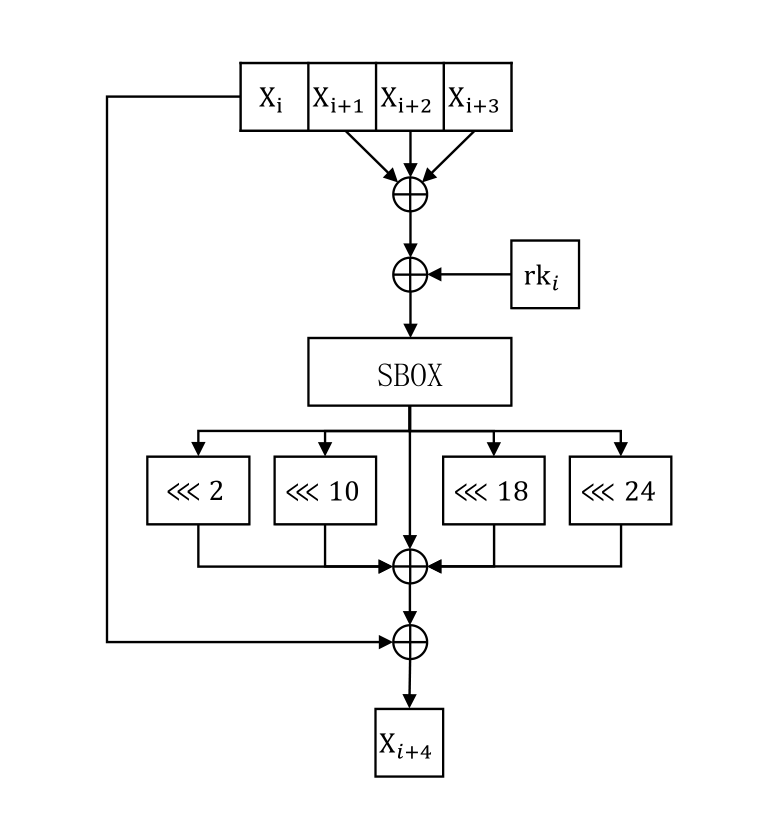
\includegraphics[width=0.8\textwidth]{sm4加密轮函数算法.png}
					\caption{加密轮函数流程图}
					\label{fig:round_crypt_flow_chart}
				\end{figure}
			
				轮函数的伪代码如\cref{alg:sm4_round_function}所示。
				
				\begin{algorithm}
					\caption{加密轮函数}
					\label{alg:sm4_round_function}
					\begin{algorithmic}[1]
						\Require $input[128],rk[32]$
						\Ensure $output[32]$
						\Function{SM4RoundFunction}{$input, rk$}
						\State $state\gets \Call{XOR}{input[32:63], input[64:95], input[96:127], rk}$;
						\State $state\gets \Call{SBOX}{state}$;
						\State $state\gets \Call{XOR}{input[0:31], state, state\lll 2, state\lll 10, state\lll 18, state\lll 24}$;
						\State $output\gets state$;
						\State \Return{$output$}
						\EndFunction
					\end{algorithmic}
				\end{algorithm}
			
				将轮函数$F$的过程用数学公式可表示为:
				$$F(X_0, X_1, X_2, X_3, rk)=X_0\oplus T(X_1\oplus X_2\oplus X_3\oplus rk)$$
				设 $B=X_1\oplus X_2\oplus X_3\oplus rk$,则有:
				\begin{align*}
					F(X_0, X_1, X_2, X_3, rk)=&X_0\oplus [SBOX(B)]\oplus [SBOX(B)\lll 2] \oplus [SBOX(B)\lll 10]\\&\oplus [SBOX(B)\lll 18]\oplus [SBOX(B)\lll 24]
				\end{align*}
			\subsubsection{加密算法}
				加密算法的整体流程图如\cref{fig:crypt_flow_chart}所示。
				\begin{figure}[htbp]
					\centering
					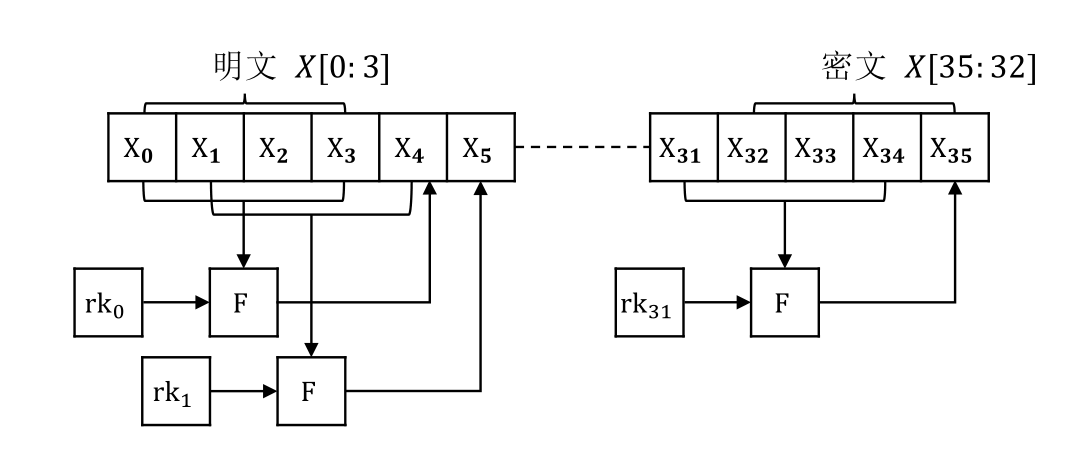
\includegraphics[width=\textwidth]{sm4加密算法.png}
					\caption{加密算法整体流程图}
					\label{fig:crypt_flow_chart}
				\end{figure}
				
				其伪代码如\cref{alg:sm4_encrypt_function}所示。
				\begin{algorithm}
					\caption{加密算法}
					\label{alg:sm4_encrypt_function}
					\begin{algorithmic}[1]
						\Require $input[128],key[128]$
						\Ensure $output[128]$
						\Function{SM4EncryptFunction}{$input, key$}
						\State $rk\gets \Call{KeyExpansion}{key}$;
						\State $state\gets input$;
						\For{$i=0\to 31$}
							\State $state \gets state[32:127] + \Call{SM4RoundFunction}{state, rk[i]}$;
						\EndFor
						\State $output\gets state[96:127] + state[64:95] + state[32:63] + state[0:31]$;
						\State \Return{$output$}
						\EndFunction
					\end{algorithmic}
				\end{algorithm}
				
				设明文为$(X_i, X_{i+1}, X_{i+2}, X_{i+3})$,4个32位数字,轮密钥$rk_i$为1个32位数字。则加密算法可用数学公式表示如下:
				$$X_{i+4}=F(X_i, X_{i+1}, X_{i+2}, X_{i+3},rk_i)$$
				
				SM4算法每次取最后四个结果与轮函数进行计算,得到下一个运算结果。经过32轮计算后,取最后四个32位数字,将其进行反转,即可得到密文。
			\subsubsection{解密算法}
				SM4的解密算法流程与加密算法完全相同,只需要将所有轮密钥反向使用即可。要证明这一点,仅需证明$$F(X_{i+4},X_{i+3},X_{i+2},X_{i+1}, rk_i) = X_i$$
				
				根据轮密钥公式,可知
				$$F(X_{i+4},X_{i+3},X_{i+2},X_{i+1}, rk_i)=X_{i+4}\oplus T(X_{i+1}\oplus X_{i+2}\oplus X_{i+3}\oplus rk_i)$$
				
				因为加密时有
				$$X_{i+4}=X_{0}\oplus T(X_{i+1}\oplus X_{i+2}\oplus X_{i+3}\oplus rk_i)$$
				
				所以(令$B=X_{i+1}\oplus X_{i+2}\oplus X_{i+3}\oplus rk_i$)有
				$$F(X_{i+4},X_{i+3},X_{i+2},X_{i+1}, rk_i)=X_{i+4}\oplus T(B)\oplus T(B)=X_i$$
				
				证毕。
			\subsubsection{轮密钥扩展}
				轮密钥扩展算法的流程图如\cref{fig:key_expension_flow_chart}所示。
				\begin{figure}[htbp]
					\centering
					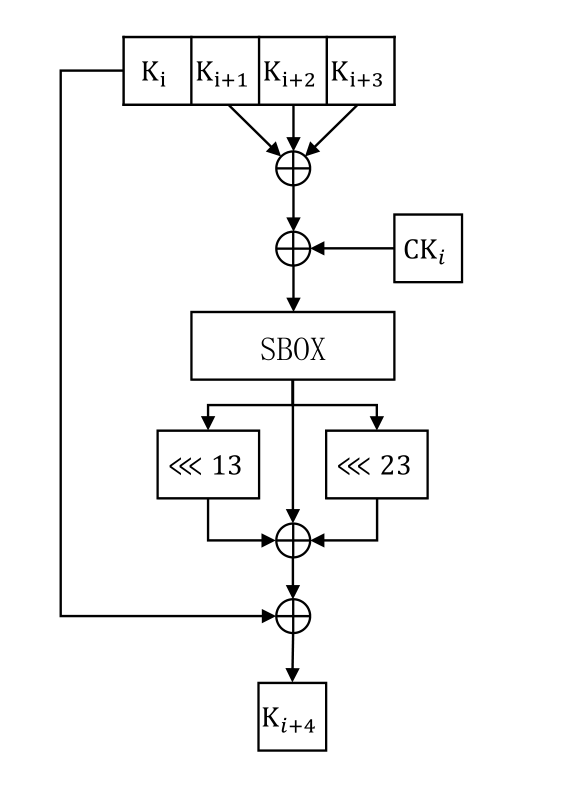
\includegraphics[width=0.7\textwidth]{sm4轮密钥扩展算法.png}
					\caption{轮密钥扩展算法流程图}
					\label{fig:key_expension_flow_chart}
				\end{figure}
				
				其伪代码如\cref{alg:key_expension_function}所示。
				\begin{algorithm}
					\caption{轮密钥扩展算法}
					\label{alg:key_expension_function}
					\begin{algorithmic}[1]
						\Require $key[128]$
						\Ensure $rk[32][32]$
						\Function{SM4EncryptFunction}{$key$}
						\State $state\gets key\oplus FK$;
						\For{$i=0\to 31$}
							\State $tmp\gets state[32:63]\oplus state[64:95]\oplus state[96:127]\oplus CK[i]$;
							\State $state \gets state[32:127] + (tmp\oplus (tmp\lll 13)\oplus (tmp\lll 23))$;
							\State $rk[i] = state[96:127]$
						\EndFor
						\State \Return{$rk$}
						\EndFunction
					\end{algorithmic}
				\end{algorithm}
				其中,$FK$与$CK$分别为系统参数与固定参数,其计算过程与加密算法十分相似。这样生成的轮函数涉及到了大量的非线性运算,可以更好地抵御线性攻击,提高轮密钥的安全性。
			\subsection{PKCS7填充}
				\subsubsection{简介}
				PKCS7也成为加密消息的语法标准,是由RSA安全体系在公钥加密系统中交换数字证书产生的一种加密标准。PKCS7标准定义中,规定的填充模式为填充字符串由一个字节序列组成,每个字节填充该填充字节序列的长度;如果数据恰好与分组对齐,则填充长度为分组大小的数据。这虽然牺牲了数据长度,但解密方却可以更加灵活透明的去解包数据。

				使用PKCS7填充的好处在于,最后一个字节肯定为填充数据的长度,所以在解密后可以准确地删除填充的数据。同时,如果填充部分在解密出现问题,可以轻易地被解密方发现。
				\subsubsection{算法流程}
				其具体方法为,首先计算当前长度,随后根据块大小得出填充区大小,并在当前字符串后追加填充字符。若恰好无需填充,为确保解密后可以正确删除填充,要求再填充一个块。其伪代码如\cref{alg:PKCS7}所示。
				\begin{algorithm}
					\caption{PKCS7填充}
					\label{alg:PKCS7}
					\begin{algorithmic}[1]
						\Require $data, BlockSize$
						\Ensure $output$
						\Function{PKCS7Padding}{$data, BlockSize$}
						\State $PaddingSize\gets BlockSize - (\Call{length}{data}\mod BlockSize$);
						\State $Padding\gets \Call{Byte}{PaddingSize} \times PaddingSize$;
						\State $output \gets data + Padding$
						\State \Return{$output$}
						\EndFunction
					\end{algorithmic}
				\end{algorithm}
			\subsection{加密模式}
				\subsubsection{密码本模式}
					电码本模式(Electronic Codebook Book, ECB)是最为简单的模式。只需要将整个明文按照分组长度进行分组,对每一组进行单独加密即可。
					
					这样的工作模式并不安全。由于相同的明文块对应了相同的密文块,因此不能很好的隐藏数据。对于特定形式的明文,如果明文中有大量周期性重复的元素,或者具有特定的结构,攻击者可以快速确定这些元素,并获取部分或完整的明文。
					
					ECB工作模式下,SM4加密函数调用图如\cref{fig:ecb-sm4-function}所示。
					\begin{figure}[htbp]
						\centering
						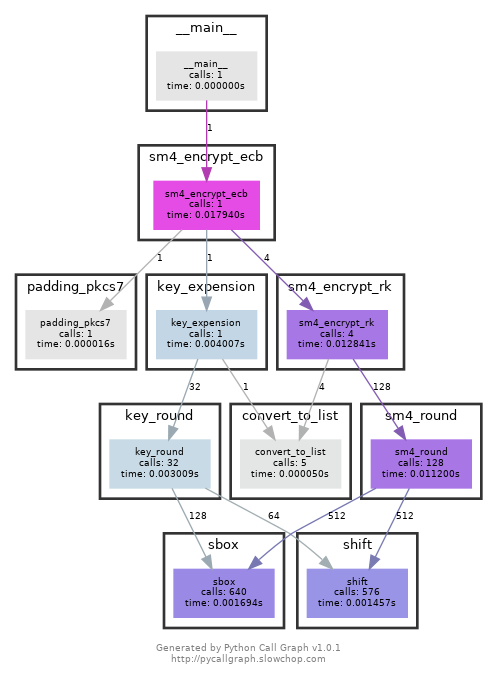
\includegraphics[width=0.7\textwidth]{ecb模式加密函数调用图.png}
						\caption{ECB工作模式下SM4加密算法函数调用图}
						\label{fig:ecb-sm4-function}
					\end{figure}
				\subsubsection{密码分组链接模式}
					密码分组链接模式(Cipher Block Chaining, CBC)首先将明文进行分组,然后每一组首先与上一组的加密结果继续异或运算后,再与密钥进行加密。其加解密流程图如\cref{fig:CBC_crypt_flow}所示。
					
					\begin{figure}[htbp]
						\centering
						\subfigure[加密模式]{
							\includegraphics[width=0.45\textwidth]{CBC加密模式.png}
							\label{subfig:CBC_encrypt}
						}
						\subfigure[解密模式]{
							\includegraphics[width=0.45\textwidth]{CBC解密模式.png}
							\label{subfig:CBC_decrypt}
						}
						\caption{CBC工作模式流程图}
						\label{fig:CBC_crypt_flow}
					\end{figure}
					
					这种加密方式是最为常用的工作模式。其优点为,每个密码分组不仅仅依赖于当前明文,也与此前所有数据的分组均有关;其缺点为,加密时由于依赖于前一个密文,无法进行并行运算,只能进行串行。而解密时由于所有密文都已知,可以进行并行计算。
					
					CBC工作模式下,SM4加密函数调用图如\cref{fig:cbc-sm4-function}所示。
					\begin{figure}[htbp]
						\centering
						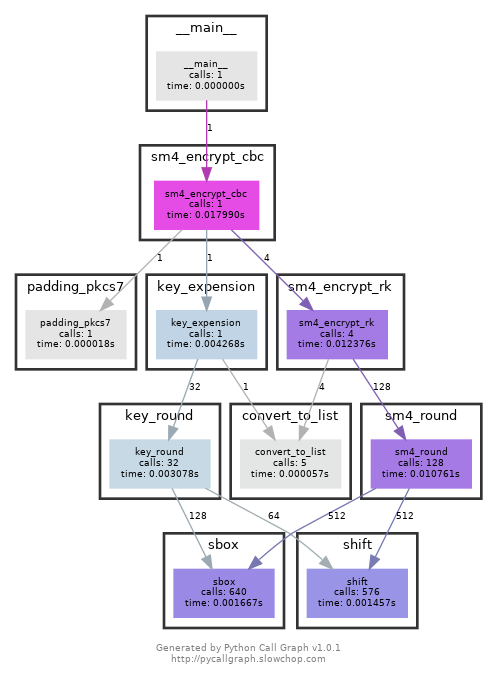
\includegraphics[width=0.7\textwidth]{cbc模式加密函数调用图.png}
						\caption{CBC工作模式下SM4加密算法函数调用图}
						\label{fig:cbc-sm4-function}
					\end{figure}
				\subsubsection{计数器模式}
					计数器模式(Counter, CTR)使用了一个自增的算子,使用加密算法对该算子进行加密后,用其结果与明文直接进行异或运算,得到密文。这样就相当于把块密码转换为了流密码,可以进行并行的加解密。
					
					而计数器模式中,可能存在的问题为每次重新启动时,要确保初始的计数器值并不相等,否则通过一些简单的异或运算,即可计算出明文。
					CTR工作模式下,SM4加密函数调用图如\cref{fig:ctr-sm4-function}所示。
					\begin{figure}[htbp]
						\centering
						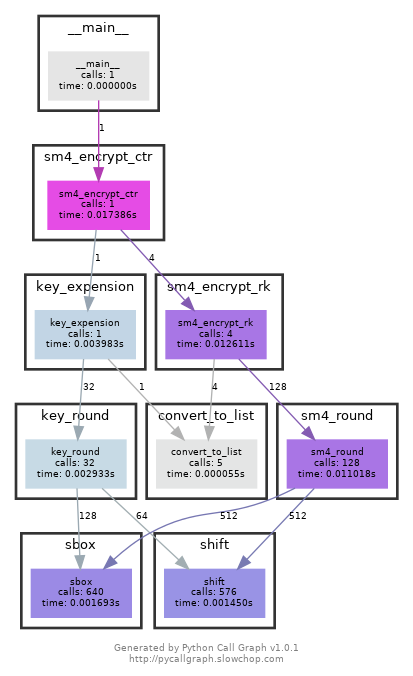
\includegraphics[width=0.6\textwidth]{ctr模式加密函数调用图.png}
						\caption{CTR工作模式下SM4加密算法函数调用图}
						\label{fig:ctr-sm4-function}
					\end{figure}
			\subsection{针对PKCS7填充和CBC加密模式的填充攻击}
				\subsubsection{填充攻击简介}
					加密服务器的填充攻击(Padding Oracle Attack)是针对一个使用固定填充算法并在加密解密中使用固定密钥的服务器的黑盒攻击。填充攻击通过向服务器发送特殊构造的密文,并接收服务器解密后填充正确或填充错误的反馈信息,以此来检查密文信息的填充。因此,进行填充攻击需要满足如下前提条件:
					\begin{enumerate}[1.]
						\item 解密服务器总是使用某个固定的密钥K,使用某个固定的填充方法PAD。
						\item 攻击者可以访问解密服务器,并且能够选择任意的合法输入消息,最后可以获得解密结果是否符合填充要求的信息。
						\item 攻击者可以获得密文以及初始化向量iv。
					\end{enumerate}
				\subsubsection{针对PKCS7填充的攻击方式}
					根据\cref{subfig:CBC_decrypt}所示的CBC模式解密流程,可以发现,只要可以对iv进行修改,攻击者就可以构造任意的解密结果。虽然服务器不会将解密结果返回给攻击者,但会告知攻击者,他所提供的密文能否被正常解密,例如,当填充出现错误时,服务器可能会抛出HTTP 500等异常,而填充正确时,则会返回200或300等结果。\upcite{1, 2}
					
					根据服务器的特点,攻击者就可以通过小范围的爆破,枚举出正确的填充。
					
					其具体操作方式如下:
					\begin{enumerate}[1.]
						\item 枚举填充:对iv的最后一个字节进行枚举,直到满足填充要求;
						\item 迭代更新:此时最后一位的填充应为01,对最后一位iv异或01和02;
						\item 枚举填充:对iv的倒数第二个字节进行枚举,直到满足填充要求;
						\item 迭代更新:此时后两位的填充均为02,对最后两位iv异或02和03;
						\item 重复进行枚举和更新,直到成功将一组中所有的字节填充满;
						\item 此时有$m\oplus iv=\mathrm{PKCS7}(block)$,对构造的iv每一位异或分组大小,随后与原始iv进行异或,即可得到明文。
					\end{enumerate}
				
					上述步骤为一个适用范围较广的解法,但其中却具有一定的问题。当明文具有填充位时,第一轮填充攻击的结果并不一定使得最后的填充长度为1。例如,求解出的明文与当时的iv异或后,末尾两个字节可能恰好为0202,同样满足填充要求,但此时攻击者由于无法直接得知解密结果,会误以为结尾的填充仍然为1,最终攻击失败。
					
					为了解决这个问题,在对最后一位进行枚举时,记录所有可能的结果(由于前面的iv并未发生修改,因此最多记录两个数字)。若最后仅记录一个数字,则该数字对应的填充一定为1,可进行正常的攻击。由于前面的部分不会受到影响,最多记录两个数字,其中一个对应着填充长度为1,另一个对应着原始填充长度,不妨设记录的数字为$k_1,k_2$,解密结果为$a$,则有
					$$a\oplus k_1=x$$ $$a\oplus k_2=1$$
					可得$x=k_1\oplus k_2\oplus 1$,从而得到已经符合要求的填充长度,那么这一部分的填充无需再进行爆破,可以直接跳转到已填充好的位置前进行爆破攻击。这样操作即提高了算法的适用范围,也可以在一定情况下节省枚举的次数,加快算法速度。
					
					然而,对于获得的两个iv方案,为了进行排除,需要从中选择一个,对该iv的倒数第二个字节进行爆破填充为2的爆破,若爆破成功,则说明这个iv对应的填充为1,这是选择另一个iv即可。对于填充长度为2时,由于异或后结尾为1,对所有的爆破都能成功,因此需要把筛选条件成爆破全部失败修改为爆破全部成功。这样就可以确定已有的iv了。
					
					在对算法进行了以上修改后,可以直接在原始的iv进行构造,而无需在一个全0上进行构造,这样当面对结尾有填充或者格式与填充相同的明文时,可以快速跳过填充部分,节省时间。
					
					\subsubsection{另一种针对特殊情况的处理方案}
					
					经过与助教的讨论后,发现面对特殊数据时,有另一个处理更加简单,但效率较低的解决方案。其主要方案为大致为,在对每一位的爆破中均记录下所有填充为正确的结果,如果结果数量大于一个,说明该位存在两种爆破方案,而第二种爆破方案一定是因为前一个字节的明文结果较为特殊,恰好构成了填充,此时,可以直接对自己构造的iv进行更改,将前一个字节的iv值修改后,重新爆破,这样前一个字节特殊明文就会被修改,无法影响到这一位填充的正常爆破。
					
					而实际上,多种可能性的情况只可能出现在最后一字节中,因为一旦最后一字节确定,当前的填充长度就是确定的,不会被前面的字节所影响。
					
					因此,这个方案相较于上一节中提及的方案,实现起来更加简单,且代码的可阅读性更强,但缺点在于,只能一位一位进行爆破,且可能出现一位多次爆破的可能性,比起上一节中可以跳过已有填充的方案,效率更低。
			\subsection{测试样例及结果截图}
			测试样例见\cref{apx:testdata}中的\cref{lst:sm4testdata},其在WSL Ubuntu控制台中的运行结果如\cref{fig:sm4_console_res}所示。
			
			\begin{figure}[htbp]
				\centering
				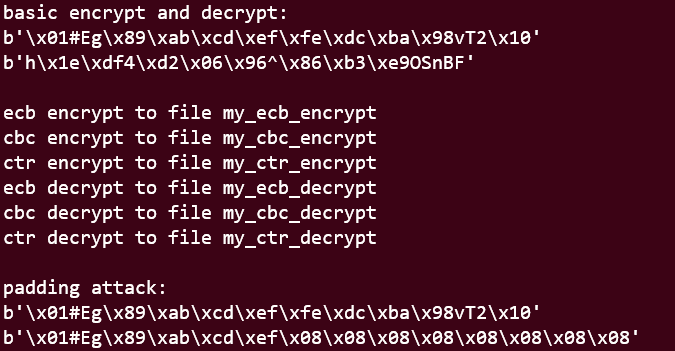
\includegraphics[width=\textwidth]{sm4控制台结果截图.png}
				\caption{测试样例运行结果截图}
				\label{fig:sm4_console_res}
			\end{figure}

			加密结果与正确的密文结果的比较,如\cref{fig:sm4_encrypt}所示。

			\begin{figure}[htbp]
				\centering
				\subfigure[ECB工作模式加密结果对比]{
					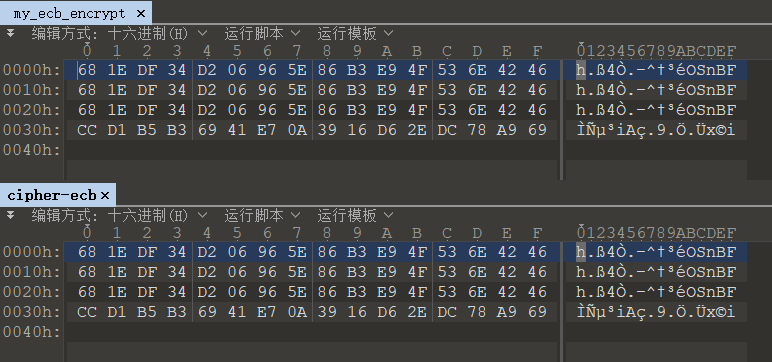
\includegraphics[width=0.9\textwidth]{sm4ecb加密截图.png}
					\label{subfig:sm4_ecb_encrypt}
				}
				\subfigure[CBC工作模式加密结果对比]{
					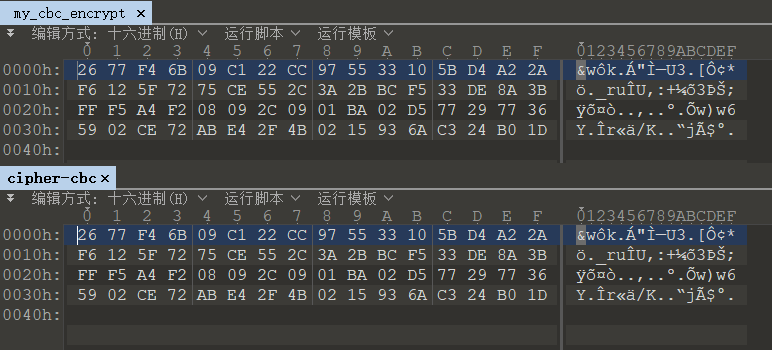
\includegraphics[width=0.9\textwidth]{sm4cbc加密截图.png}
					\label{subfig:sm4_cbc_encrypt}
				}
				\subfigure[CTR工作模式加密结果对比]{
					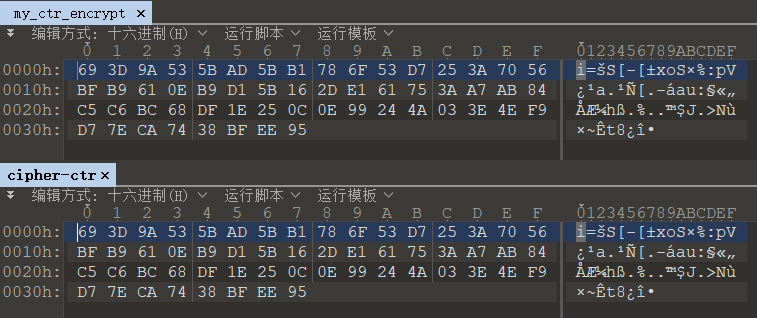
\includegraphics[width=0.9\textwidth]{sm4ctr加密截图.png}
					\label{subfig:sm4_ctr_encrypt}
				}
				\caption{各工作模式加密结果对比}
				\label{fig:sm4_encrypt}
			\end{figure}

			解密结果与正确结果message的比较,如\cref{fig:sm4_decrypt}所示。

			\begin{figure}[htbp]
				\centering
				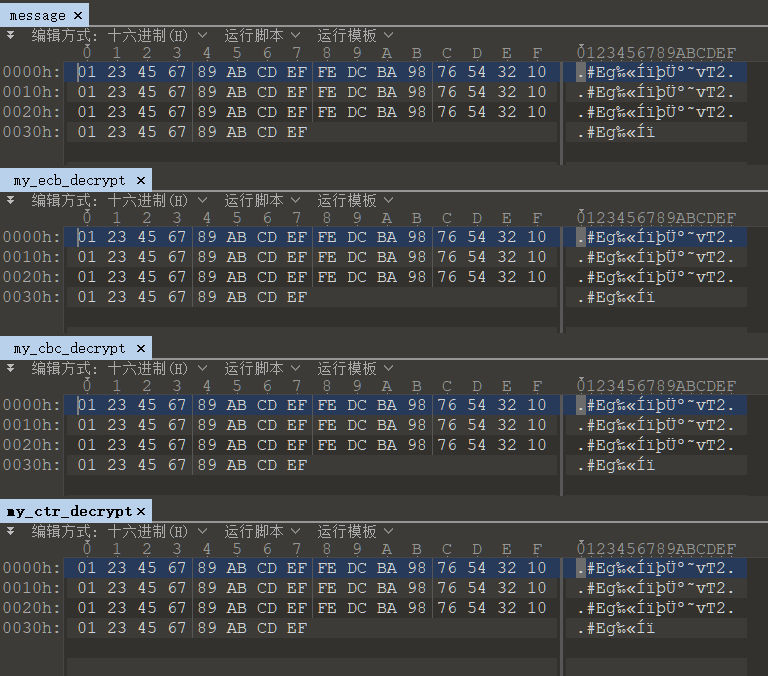
\includegraphics[width=\textwidth]{sm4解密截图.png}
				\caption{各工作模式解密结果对比}
				\label{fig:sm4_decrypt}
			\end{figure}

			Padding Oracle Attack攻击结果如\cref{fig:sm4_console_res}中padding attack部分所示。分别进行两组测试,且两组数据均来自文件“cipher\_cbc”第一行为无填充的常规情况,第二行为末尾有8个字节PKCS7填充的特殊情况,两组测试结果均正常。
			
		\section{收获与建议}
			由于本次实验所使用的sm4算法处理较为复杂,并且在开始时并未对代码的数据类型做好规划,这就导致了数据类型在使用中多次转换的混乱现象。在后续的实验中,应当汲取教训,规范好各个模块的数据类型,避免出现数据类型在整型、字节中多次转换的现象,增强程序的可读性,提高程序的效率。

			尝试进行Padding Oracle Attack时,仿照着论文中的流程进行编程,但在测试时发现对于特殊情况(结尾已有填充或者除最后字节外与填充相似)程序因为无法确认最后一个字节,可能会出现爆破错误的情况。在此基础上,对其原理及出现问题的地方进行了分析,最终选择将最后一字节的确定单独取出,进行完整的爆破流程,并对所有可能结果(1-2种可能)进行分析,以此来确定了最后一个字节,并明确了现有填充长度,节省了爆破的空间,实现了对算法的优化。
		\newpage
		\begin{thebibliography}{99}
			\bibitem{1}
			Katz J, Lindell Y. Introduction to modern cryptography[M]. CRC press, 2020.
			\bibitem{2}
			flurry. Padding oracle attack详细解析[EB/OL]. (2017-10-25)[2021-04-27]. https://www.freebuf.com/articles/database/151167.html.
		\end{thebibliography}
		\newpage
		\appendix
			\section{测试样例}\label{apx:testdata}
			\begin{lstlisting}[caption={SM4实验测试样例}, label={lst:sm4testdata}]
import CNSPP

test = [0x681EDF34D206965E86B3E94F536E4246, 0x123456789abcdeffedcba9876543210]

print ('basic encrypt and decrypt:')
print (CNSPP.sm4_decrypt(test[0], test[1]))
print (CNSPP.sm4_encrypt(test[1], test[1]))

plain = open('message', 'rb').read()
print ('\necb encrypt to file my_ecb_encrypt')
open('my_ecb_encrypt', 'wb').write(CNSPP.sm4_encrypt_ecb(plain, test[1]))

print ('cbc encrypt to file my_cbc_encrypt')
open('my_cbc_encrypt', 'wb').write(CNSPP.sm4_encrypt_cbc(plain, test[1], test[1]))

print ('ctr encrypt to file my_ctr_encrypt')
open('my_ctr_encrypt', 'wb').write(CNSPP.sm4_encrypt_ctr(plain, test[1], test[1]))

print ('ecb decrypt to file my_ecb_decrypt')
open('my_ecb_decrypt', 'wb').write(CNSPP.sm4_decrypt_ecb(open('cipher-ecb', 'rb').read(), test[1]))

print ('cbc decrypt to file my_cbc_decrypt')
open('my_cbc_decrypt', 'wb').write(CNSPP.sm4_decrypt_cbc(open('cipher-cbc', 'rb').read(), test[1], test[1]))

print ('ctr decrypt to file my_ctr_decrypt')
open('my_ctr_decrypt', 'wb').write(CNSPP.sm4_decrypt_ctr(open('cipher-ctr', 'rb').read(), test[1], test[1]))

print ('\npadding attack:')
print (CNSPP.padding_attack(
	b'\xF6\x12\x5F\x72\x75\xCE\x55\x2C
	\x3A\x2B\xBC\xF5\x33\xDE\x8A\x3B
	\xFF\xF5\xA4\xF2\x08\x09\x2C\x09
	\x01\xBA\x02\xD5\x77\x29\x77\x36', test[1]))
print (CNSPP.padding_attack(
	b'\xFF\xF5\xA4\xF2\x08\x09\x2C\x09
	\x01\xBA\x02\xD5\x77\x29\x77\x36
	\x59\x02\xCE\x72\xAB\xE4\x2F\x4B
	\x02\x15\x93\x6A\xC3\x24\xB0\x1D', test[1]))
				
			\end{lstlisting}
\end{document}